\chapter{La Gestion Actif-Passif et le Modèle de Simulation en Python}

\section{Principes et Enjeux de la Gestion Actif-Passif (ALM)}
La gestion Actif-Passif (ALM) trouve son origine dans une particularité fondamentale du secteur de l'assurance énoncé précédemment dans le mémoire : le \textbf{cycle de production inversé}. Contrairement à une entreprise classique qui vend un produit avant d'en percevoir le revenu, un assureur collecte des primes aujourd'hui en échange de la promesse de verser des prestations dans un futur lointain et incertain. Ce décalage temporel est au cœur du modèle économique de l'assurance vie.

Ce mécanisme engendre une inadéquation structurelle (\textit{mismatch}) entre les deux côtés du bilan. D'une part, le passif est constitué d'engagements de longue durée, dont l'échéance et le montant sont soumis à des aléas (mortalité, comportement de rachat des assurés). D'autre part, pour couvrir ces engagements, l'assureur investit les primes sur les marchés financiers, constituant un actif dont la valeur et les flux sont, par nature, volatiles et dépendants du contexte économique.

Cette inadéquation est renforcée par une interdépendance dynamique et complexe entre l'actif et le passif.

\begin{itemize}
    \item \textbf{Le passif influe sur l'actif :} Le versement des prestations (rachats, décès) contraint l'assureur à liquider une partie de ses actifs, parfois dans des conditions de marché défavorables.
    \item \textbf{L'actif influe sur le passif :} La performance des actifs financiers a un impact direct sur le niveau des engagements. C'est notamment le cas de la \textbf{Participation aux Bénéfices (PB)}, qui dépend des résultats financiers générés par l'assureur. Le Code des assurances impose une redistribution minimale aux assurés, calculée comme suit :
    \begin{equation}
        \label{eq:pb_minReg}
        \text{PB}_{\text{minReg}} = 85\% \times \max(\text{RésFi}, 0) + 
        \begin{cases}
            90\% \times \text{RésTech} & \text{si RésTech} \ge 0 \\
            100\% \times \text{RésTech} & \text{si RésTech} < 0
        \end{cases}
    \end{equation}
    Où le Résultat Financier (RésFi) est directement issu de la performance des actifs et le Résultat Technique (RésTech) des risques de mortalité et de rachat.
\end{itemize}
La gestion Actif-Passif est donc la discipline qui vise à piloter les risques nés de cette interdépendance afin d'assurer la solvabilité et d'optimiser la rentabilité de l'acteur.

\subsection{La Modélisation ALM : un Outil de Projection Essentiel}

Pour quantifier et piloter les risques complexes découlant de l'inadéquation actif-passif, les assureurs ont recours à des modèles de projection actuariels sophistiqués, communément appelés modèles de Gestion Actif-Passif ou modèles ALM. L'utilité principale de ces modèles est de projeter le bilan d'un assureur, qu'il s'agisse d'un bilan prudentiel sous Solvabilité 2 ou d'un bilan comptable sous les normes IFRS17, afin d'évaluer la santé financière future de l'organisme sur un horizon de long terme. Leur fonctionnement repose sur la combinaison de deux piliers fondamentaux : des scénarios prospectifs sur l'environnement économique et financier, et des hypothèses sur le comportement futur des assurés (lois de mortalité, de rachat, etc.).

L'approche de modélisation peut être déterministe ou stochastique, chaque approche répondant à des objectifs d'analyse distincts.

L'approche \textbf{déterministe} consiste à projeter le bilan de l'assureur selon une trajectoire unique et prédéfinie de l'environnement économique. Cette trajectoire, qualifiée de \textbf{scénario central}, est généralement construite à partir de la courbe des taux sans risque fournie par l'EIOPA. Elle permet d'obtenir le (\textit{Best Estimate}) central, c'est à dire la somme des flux futurs actualisés du portefeuille dans un contexte économique considéré comme le plus probable, servant de base pour le plan d'affaires et la valorisation prudentielle.

Cependant, une approche déterministe ne peut à elle seule capturer l'éventail des risques, notamment ceux liés aux options et garanties financières (par exemple, les Taux Minimum Garantis ou les options de rachat) dont le coût ne se matérialise que dans des conditions de marché adverses. Pour pallier cette limite, une approche \textbf{stochastique} est nécessaire. Celle-ci s'appuie sur un \textbf{Générateur de Scénarios Économiques (GSE)} pour simuler un grand nombre (souvent plusieurs milliers) de trajectoires économiques futures possibles, chacune représentant une évolution plausible des marchés financiers.

Chaque scénario économique généré sert alors d'input pour une projection complète du modèle ALM. En agrégeant les résultats de ces multiples projections via la \textbf{méthode de Monte Carlo}, l'assureur obtient non plus une seule valeur, mais une distribution des résultats possibles. L'objectif final est de disposer, pour chaque trajectoire, du détail des flux financiers à la maille la plus fine. Cette granularité permet une analyse statistique approfondie des risques, comme le calcul de quantiles (Value at Risk à 99.5\%) pour déterminer le capital de solvabilité requis (SCR) sous Solvabilité 2. Ces modèles stochastiques sont donc au cœur de l'évaluation des risques et de la prise de décision stratégique, et constituent le fondement du modèle de simulation qui sera détaillé dans la suite de ce chapitre.

\begin{figure}[H]
    \centering
    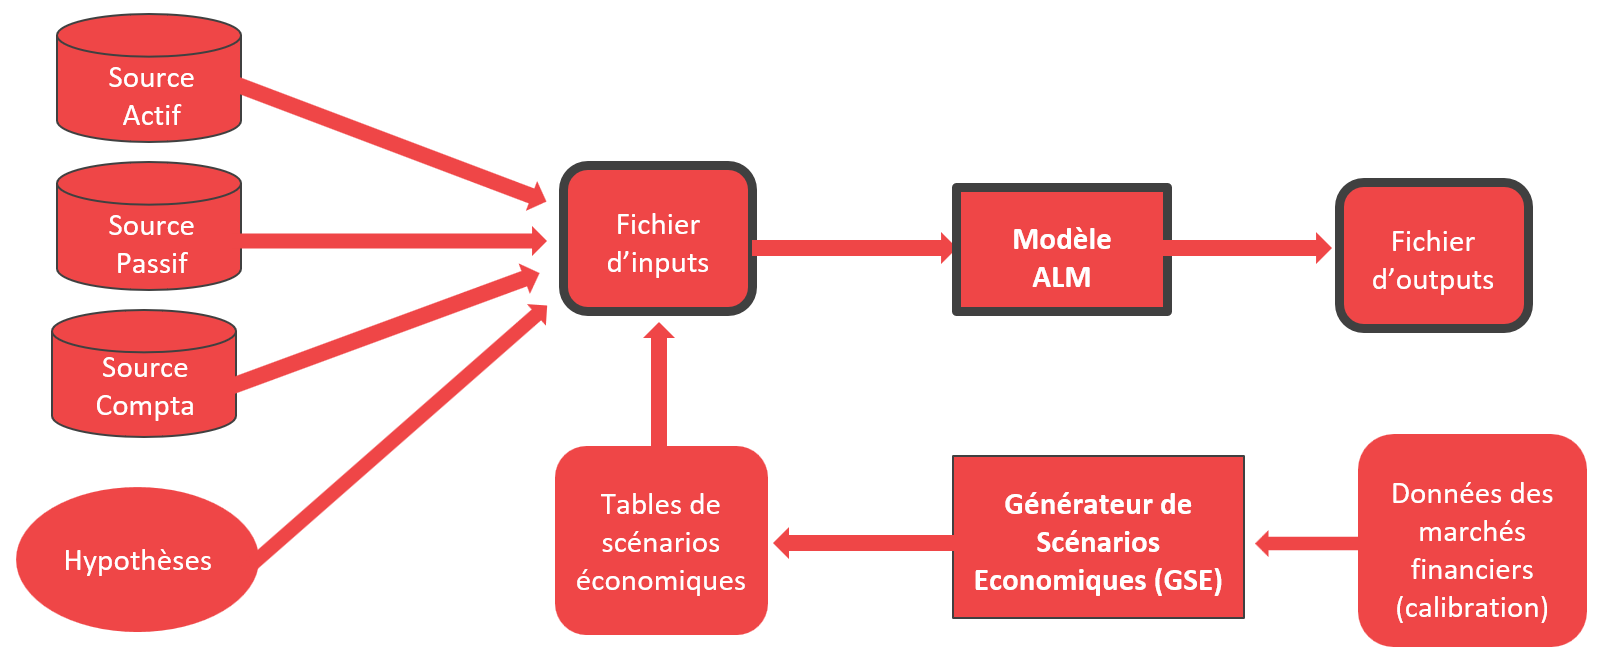
\includegraphics[width=0.8\textwidth]{images/2_chapitres/chapitre2/alm_det.png}
    \caption{Fonctionnement d'un modèle ALM \textbf{(graphique temporaire)}}
    \label{fig:alm_det}
\end{figure}



\section{Architecture et Fonctionnement du Modèle de Projection}
Dans cette partie, le fonctionnement détaillé du modèle ALM développé en Python pour Accenture sera présenté. Ce modèle vise à projeter de manière conjointe l'actif et le passif d'un assureur vie sur un horizon de long terme, en intégrant les interactions complexes entre les deux, ainsi que les stratégies de gestion d'actifs et de participation aux bénéfices. Le modèle est structuré autour de plusieurs modules clés, chacun responsable d'une composante spécifique de la projection.

Cette partie n'est pour le moment pas encore terminée. Il sera question de détailler les mécanismes de projection du passif, de projection de l'actif, ainsi que l'interaction entre les deux ainsi que les limitations actuelles du modèle. Dans cette partie je vais également expliquer en détail comment sont calculer BE, SCR et PVFP qui sont les pierres angulaires dans les analyses de ce mémoire.

    \subsection{Projection du Passif}
    % Votre texte ici...
    \subsection{Projection de l'Actif}
    % Votre texte ici...
    \subsection{Interaction Actif-Passif : Stratégie d'Investissement et Politique de Participation aux Bénéfices (PB)}
    % Votre texte ici...

\section{Limites Actuelles du modèle}
A date, les fonds propres ne sont pas modélisés dans le modèle ALM. En effet, le modèle se concentre sur la projection de l'actif et du passif, ainsi que sur les interactions entre les deux, mais n'intègre pas encore la dynamique des fonds propres. Cette limitation est importante car les fonds propres jouent un rôle crucial dans la solvabilité et la résilience financière de l'assureur. Leur modélisation permettrait de mieux évaluer l'impact des stratégies de gestion sur la solidité financière globale de l'entreprise. L'absence des fonds propres nous empêche de calculer des indicateurs cruciaux tels que le ratio de solvabilité.

% \chapter{La Gestion Actif-Passif et développement d'un modèle ALM en Python}
% \section{La gestion Actif-Passif (ALM) : définitions et enjeux}
% \label{sec:alm}

% \subsection{Le cycle de production inversé, origine de l'inadéquation Actif-Passif}

% La gestion Actif-Passif (ALM) trouve son origine dans une particularité fondamentale du secteur de l'assurance que l'on a énoncé dans le début de ce chapitre : le \textbf{cycle de production inversé}. Contrairement à une entreprise classique qui vend un produit avant d'en percevoir le revenu, un assureur collecte des primes aujourd'hui en échange de la promesse de verser des prestations dans un futur lointain et incertain. Ce décalage temporel est au cœur du modèle économique de l'assurance vie.

% Ce mécanisme engendre une inadéquation structurelle (\textit{mismatch}) entre les deux côtés du bilan. D'une part, le passif est constitué d'engagements de longue durée, dont l'échéance et le montant sont soumis à des aléas (mortalité, comportement de rachat des assurés). D'autre part, pour couvrir ces engagements, l'assureur investit les primes sur les marchés financiers, constituant un actif dont la valeur et les flux sont, par nature, volatiles et dépendants du contexte économique.

% Cette inadéquation est renforcée par une interdépendance dynamique et complexe entre l'actif et le passif.

% \begin{itemize}
%     \item \textbf{Le passif influe sur l'actif :} Le versement des prestations (rachats, décès) contraint l'assureur à liquider une partie de ses actifs, parfois dans des conditions de marché défavorables.
%         \item \textbf{L'actif influe sur le passif :} La performance des actifs financiers a un impact direct sur le niveau des engagements. C'est notamment le cas de la \textbf{Participation aux Bénéfices (PB)}, qui dépend des résultats financiers générés par l'assureur. Le Code des assurances impose une redistribution minimale aux assurés, calculée comme suit :
%         \begin{equation}
%             \label{eq:pb_minReg}
%             \text{PB}_{\text{minReg}} = 85\% \times \max(\text{RésFi}, 0) + 
%             \begin{cases}
%                 90\% \times \text{RésTech} & \text{si RésTech} \ge 0 \\
%                 100\% \times \text{RésTech} & \text{si RésTech} < 0
%             \end{cases}
%         \end{equation}
%         Où le Résultat Financier (RésFi) est directement issu de la performance des actifs et le Résultat Technique (RésTech) des risques de mortalité et de rachat.
% \end{itemize}
% La gestion Actif-Passif est donc la discipline qui vise à piloter les risques nés de cette interdépendance afin d'assurer la solvabilité et d'optimiser la rentabilité de l'acteur.

% \subsection{Objectifs et périmètre de l'ALM}

% % À COMPLÉTER :
% % Expliquer ici les trois grands objectifs de l'ALM :
% % 1. Maîtriser les risques (taux, marché, liquidité...).
% % 2. Assurer la solvabilité réglementaire (respect du SCR).
% % 3. Optimiser la rentabilité (maximiser le rendement pour un risque donné).


% \subsection{Le modèle ALM : un outil de simulation prospective}

% % À COMPLÉTER :
% % Décrire ici le rôle du modèle ALM comme outil de prise de décision.
% % - Principe : simulation conjointe de l'actif et du passif sur le long terme.
% % - Inputs principaux : GSE, lois de comportement, portefeuille, règles de gestion.
% % - Mentionner que vous utilisez un tel outil dans le cadre de votre mémoire, sans pour autant faire une étude ALM complète.


% \subsection{Principaux indicateurs de pilotage ALM}

% % À COMPLÉTER :
% % Lister et décrire brièvement quelques indicateurs clés issus des modèles ALM.
% % - Projection de la NAV (fonds propres prudentiels).
% % - Évolution du ratio de couverture SCR.
% % - Analyses de sensibilité et stress tests (impact d'un choc de taux, actions, etc.).

% La réalisation des analyses de sensibilités, cœur de ce mémoire, s'appuie sur un moteur de projection robuste : le modèle ALM (Asset Liability Management). Historiquement, le modèle utilisé au sein d'Accenture reposait sur une architecture en VBA (Visual Basic for Applications). Pour des impératifs de performance, de maintenabilité et de flexibilité, la décision a été prise de développer un nouveau modèle en Python. Cette migration a été l'occasion de repenser l'architecture du modèle pour mieux répondre aux exigences de calcul complexes de Solvabilité 2.

% Ce chapitre décrit ce nouveau modèle ALM. Nous présenterons son architecture globale, son fonctionnement détaillé à travers la projection des actifs, des passifs et la mise en œuvre des stratégies de gestion, et nous conclurons sur ses limites actuelles qui ouvrent des perspectives d'amélioration.

% \section{Développement du Modèle ALM en Python}

% La transition d'un modèle ALM de VBA vers Python a été motivée par la recherche de performance, de maintenabilité et de modularité. Le langage Python, avec son écosystème de librairies scientifiques comme \textit{NumPy}, \textit{Pandas} ou \textit{Polars}, offre un cadre de développement beaucoup plus robuste et performant pour des calculs actuariels intensifs.

% \subsection{Présentation du modèle ALM développé pour Accenture}

% Le modèle ALM a pour objectif principal de projeter l'ensemble des actifs et des passifs d'un assureur sur un horizon de long terme (typiquement 40 à 60 ans), sous un grand nombre de scénarios économiques stochastiques. Ces projections permettent de calculer les indicateurs prudentiels requis par la directive Solvabilité 2, notamment le BE et le SCR. Le modèle se veut un outil de pilotage stratégique, capable de simuler l'impact de différentes stratégies de gestion d'actifs, de politiques de souscription ou de participation aux bénéfices.

% \subsection{Fonctionnement du modèle ALM}

% \subsubsection{Fonctionnement général du modèle}
% Le modèle opère de manière itérative, année par année, pour chaque scénario économique. À chaque pas de temps, il simule l'ensemble des flux financiers et des opérations de bilan. Le processus global peut être résumé comme suit :
% \begin{enumerate}
% \item \textbf{Entrées :} Le modèle prend en entrée le portefeuille de passifs (issu du générateur ou d'un client), le portefeuille d'actifs, un set de scénarios économiques (ESG), et les règles de gestion (stratégie d'investissement, politique de PB, etc.).
% \item \textbf{Moteur de projection :} Pour chaque année et chaque scénario, le moteur calcule les flux de passifs, les flux d'actifs, et applique les décisions de gestion.
% \item \textbf{Sorties :} En fin de projection, le modèle génère des comptes de résultat et des bilans prévisionnels pour chaque scénario, qui sont ensuite utilisés pour calculer les indicateurs S2 par agrégation et analyse statistique.
% \end{enumerate}

% \subsubsection{Fonctionnement du passif}
% La projection du passif consiste à simuler l'évolution du portefeuille de contrats. À chaque pas de temps, le modèle calcule :
% \begin{itemize}
% \item Les primes encaissées.
% \item Les prestations versées (décès, rachats, rentes).
% \item Les chargements et frais prélevés.
% \item L'évolution des provisions mathématiques, en tenant compte de la revalorisation issue de la participation aux bénéfices.
% \end{itemize}
% Les flux de prestations sont déterminés par l'application des lois de comportement (mortalité, rachat) sur le portefeuille des assurés survivants.

% \subsubsection{Fonctionnement de l'actif}
% Simultanément, le modèle projette la valeur du portefeuille d'actifs. Pour chaque classe d'actifs (actions, obligations, immobilier, etc.), il calcule :
% \begin{itemize}
% \item L'évolution de la valeur de marché, en fonction des indices fournis par le scénario économique.
% \item Les revenus générés (dividendes, coupons, loyers).
% \end{itemize}
% Le modèle gère également le réinvestissement des flux de trésorerie et les opérations d'achat/vente décidées par la stratégie d'investissement.

% \subsubsection{Fonctionnement de la stratégie d'investissement}
% La stratégie d'investissement est un ensemble de règles qui dictent la manière dont l'actif est géré. Le modèle implémente une allocation stratégique cible (\textit{Strategic Asset Allocation} - SAA). Chaque année, il compare l'allocation réelle du portefeuille à l'allocation cible et déclenche des opérations d'achat ou de vente pour réduire l'écart, dans le respect des contraintes de liquidité et de transaction.

% \subsubsection{Fonctionnement de la stratégie ALM et de la politique de PB}
% Le cœur du modèle ALM est l'interaction entre l'actif et le passif. Le résultat financier généré par l'actif est utilisé pour déterminer la revalorisation servie aux assurés. La politique de Participation aux Bénéfices (PB) est une fonction clé qui répartit la performance financière entre l'assureur et les assurés, dans le respect des engagements contractuels et réglementaires. Le modèle simule la constitution et la reprise de la Provision pour Participation aux Bénéfices (PPB), qui permet de lisser les taux servis dans le temps.

% \subsection{Limites actuelles du modèle}
% Malgré sa robustesse, le modèle actuel présente certaines limites. Les règles de gestion, notamment la stratégie d'investissement, sont encore modélisées de manière relativement statique et ne réagissent pas toujours de façon dynamique aux conditions de marché extrêmes. De plus, la granularité de certains modules pourrait être affinée, notamment en ce qui concerne la modélisation des frais ou des impôts. Enfin, bien que les performances aient été grandement améliorées par rapport à la version VBA, les temps de calcul pour des portefeuilles très volumineux sur des milliers de scénarios restent un défi et une piste d'optimisation continue.